\documentclass[12pt]{article}

\usepackage[a4paper,margin=1in]{geometry}
\usepackage{booktabs}
\usepackage{xcolor}
\usepackage{amsmath}
\usepackage{graphicx}
\usepackage{float}
\usepackage{hyperref}

% -------------------------------------------------
% Report Details
% -------------------------------------------------

\title{
Deep Learning Laboratory\\
Assignment \#9
}

\author{
Siddharth Narayan Mishra\\
123CS0189
}

\date{\today}

\begin{document}

\maketitle

\tableofcontents

\newpage

%%%%%%%%%%%%%%%%%%%%%%%%%%%%%%%%%%%%%%%%%%%%%%%%%%%%%%%


\section*{Setup and assumptions}

The network is the fixed LeNet-style CNN from the assignment (Conv1 1$\to$6, Conv2 6$\to$16, both 5$\times$5, average pooling 2$\times$2, then FC 256-120-84-10). Training used cross-entropy, SGD with learning rate 0.01 and momentum 0.9, batch size 64, 10 epochs, seed 42 and PyTorch default initialisation. The source code and the checkpoint \texttt{lenet\_mnist.pt} are submitted separately.

Things the assignment does not fix, and what I chose:
\begin{itemize}
\item No checkpoint was provided, so I trained my own and used it unchanged for Experiments 2 to 6.
\item The 60,000 MNIST training images were split 50,000 for training and 10,000 for validation. Inputs were scaled to $[0,1]$ and normalised with mean 0.1307 and std 0.3081.
\item Section 6 says 2,000 test images, so the Top-8 scan uses a fixed random subset of 2,000 images from the MNIST test set (seed 42). Because of this, the scores and image indices here will differ from a scan over all 10,000 images.
\item No filters were assigned, so I picked them: Conv1 filter 2 (Experiment 2), Conv2 filter 7 (Experiment 3), Conv1 filters 1, 3, 5 and Conv2 filters 5, 10, 14 (Experiment 4), and Conv2 filter 3 (Experiment 6). Conv2 filter 3 was chosen because it is one of the few filters for which some images have a negative PRE-ReLU maximum, which Experiment 6 needs. Filters are numbered from 1.
\end{itemize}

Locations $(y,x)$ below are positions in the feature map (24$\times$24 for Conv1, 8$\times$8 for Conv2). The red box in the figures is the theoretical receptive field of that neuron in the 28$\times$28 input. Every activation score is the POST-ReLU value unless stated otherwise.

%%%%%%%%%%%%%%%%%%%%%%%%%%%%%%%%%%%%%%%%%%%%%%%%%%%%%%%

\section{Experiment 1: training and verification}

Table~\ref{tab:train} gives the per-epoch results. The final test accuracy is \textbf{98.55\%} on the 2,000-image test subset (98.85\% on all 10,000 test images), which is above the required 97\%.

\begin{table}[H]
\centering
\begin{tabular}{rccc}
\toprule
Epoch & Train loss & Train acc (\%) & Val acc (\%) \\
\midrule
1 & 0.4808 & 84.80 & 95.90 \\
2 & 0.0935 & 97.11 & 97.49 \\
3 & 0.0625 & 98.07 & 98.01 \\
4 & 0.0501 & 98.43 & 98.36 \\
5 & 0.0405 & 98.70 & 98.43 \\
6 & 0.0356 & 98.85 & 98.43 \\
7 & 0.0303 & 99.03 & 98.62 \\
8 & 0.0266 & 99.14 & 98.40 \\
9 & 0.0220 & 99.27 & 98.59 \\
10 & 0.0207 & 99.30 & 98.75 \\
\bottomrule
\end{tabular}
\caption{Training loss and accuracy per epoch. Training loss and accuracy are running averages over the epoch.}
\label{tab:train}
\end{table}

Output shapes (single image, batch dimension dropped):

\begin{table}[H]
\centering
\begin{tabular}{lc}
\toprule
Stage & Output shape \\
\midrule
Input & 1$\times$28$\times$28 \\
Conv1 / ReLU & 6$\times$24$\times$24 \\
AvgPool & 6$\times$12$\times$12 \\
Conv2 / ReLU & 16$\times$8$\times$8 \\
AvgPool & 16$\times$4$\times$4 \\
Flatten & 256 \\
FC1 / ReLU & 120 \\
FC2 / ReLU & 84 \\
FC3 & 10 \\
\bottomrule
\end{tabular}
\caption{Output dimension after each stage, as printed by the training script.}
\end{table}

These match the dimensions given in the assignment.

%%%%%%%%%%%%%%%%%%%%%%%%%%%%%%%%%%%%%%%%%%%%%%%%%%%%%%%

\section{Consolidated results}

For every filter, all 2,000 test images were scored with $S_i=\max_{y,x}A_i(c,y,x)$ on the POST-ReLU map and the eight highest were kept.

\begin{table}[H]
\centering
\small
\begin{tabular}{llccccl}
\toprule
Layer & Filter & Top-1 digit & Top-1 act. & Top-1 loc. & RF size & Top-8 digit distribution \\
\midrule
Conv1 & 2  & 7 & 11.97 & (5,12) & 5$\times$5   & 7:5, 2:1, 3:1, 5:1 \\
Conv2 & 7  & 2 & 11.93 & (7,7)  & 14$\times$14 & 2:7, 8:1 \\
\midrule
Conv1 & 1  & 8 & 14.42 & (21,15) & 5$\times$5   & 1:3, 4:2, 7:1, 8:1, 9:1 \\
Conv1 & 3  & 0 & 13.36 & (13,17) & 5$\times$5   & 0:4, 7:2, 9:2 \\
Conv1 & 5  & 6 & 2.72  & (1,19)  & 5$\times$5   & 6:3, 5:2, 3:1, 4:1, 9:1 \\
Conv2 & 5  & 4 & 26.50 & (1,3) & 14$\times$14 & 4:6, 0:2 \\
Conv2 & 10 & 0 & 16.89 & (6,2) & 14$\times$14 & 0:5, 2:2, 4:1 \\
Conv2 & 14 & 6 & 26.14 & (5,3)   & 14$\times$14 & 3:2, 4:2, 0:1, 2:1, 5:1, 6:1 \\
\bottomrule
\end{tabular}
\caption{Consolidated table, POST-ReLU activation. The first two rows are Experiments 2 and 3, the rest are the Experiment 4 filters.}
\label{tab:main}
\end{table}

%%%%%%%%%%%%%%%%%%%%%%%%%%%%%%%%%%%%%%%%%%%%%%%%%%%%%%%

\section{Experiment 2: Conv1 filter 2}

\begin{figure}[H]
\centering
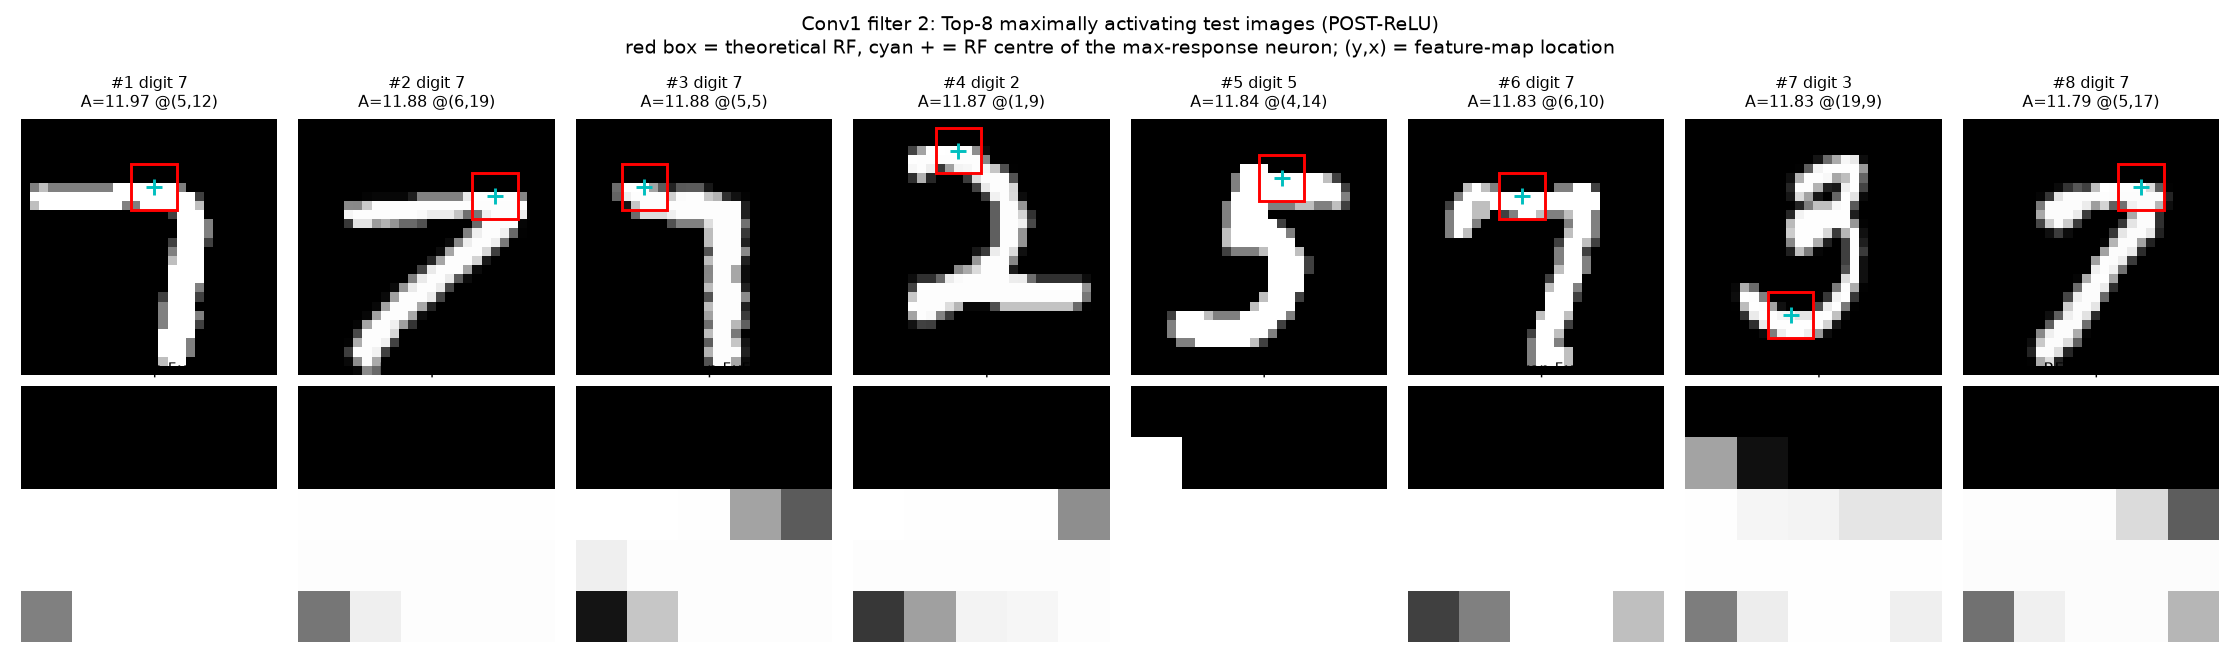
\includegraphics[width=\linewidth]{results/fig1_conv1_top8.png}
\caption{Top-8 images for Conv1 filter 2 (POST-ReLU). Red box: theoretical 5$\times$5 receptive field of the maximum-response neuron. Cyan plus: centre of that field. Bottom row: the 5$\times$5 crop.}
\label{fig:conv1}
\end{figure}

\begin{table}[H]
\centering
\small
\begin{tabular}{cccccc}
\toprule
Rank & Test idx & Digit & Score & Location $(y,x)$ & RF region (rows, cols) \\
\midrule
1 & 1515 & 7 & 11.9681 & (5,12) & 5--9, 12--16 \\
2 & 1568 & 7 & 11.8836 & (6,19) & 6--10, 19--23 \\
3 & 895  & 7 & 11.8782 & (5,5)  & 5--9, 5--9 \\
4 & 71   & 2 & 11.8709 & (1,9)  & 1--5, 9--13 \\
5 & 1387 & 5 & 11.8389 & (4,14) & 4--8, 14--18 \\
6 & 1431 & 7 & 11.8335 & (6,10) & 6--10, 10--14 \\
7 & 576  & 3 & 11.8302 & (19,9) & 19--23, 9--13 \\
8 & 1875 & 7 & 11.7861 & (5,17) & 5--9, 17--21 \\
\bottomrule
\end{tabular}
\caption{Top-8 for Conv1 filter 2. All receptive fields lie fully inside the image.}
\end{table}

\textbf{Observation.} Five of the eight images are 7s, the others are a 2, a 5 and a 3. The maximum-response location is different in every image, so the filter is not tied to one position. What the patches share is a horizontal stroke with dark background above it: in the 7s the box sits on the top bar, in the 2 and the 5 it sits on the top of the digit, and in the 3 it sits on the lower curve. In each crop the upper rows are dark and the lower rows are bright. This agrees with the kernel itself: the top two rows of its weights are mostly negative and the lower rows are positive, so it wants dark above and ink below. So this filter responds to the upper edge of a roughly horizontal stroke, and the 7s rank high mostly because a 7 has a long horizontal bar at the top. The eight scores lie in a narrow band (11.79 to 11.97), so the order within the Top-8 should not be read too closely.

%%%%%%%%%%%%%%%%%%%%%%%%%%%%%%%%%%%%%%%%%%%%%%%%%%%%%%%

\section{Experiment 3: Conv1 versus Conv2}

\begin{figure}[H]
\centering
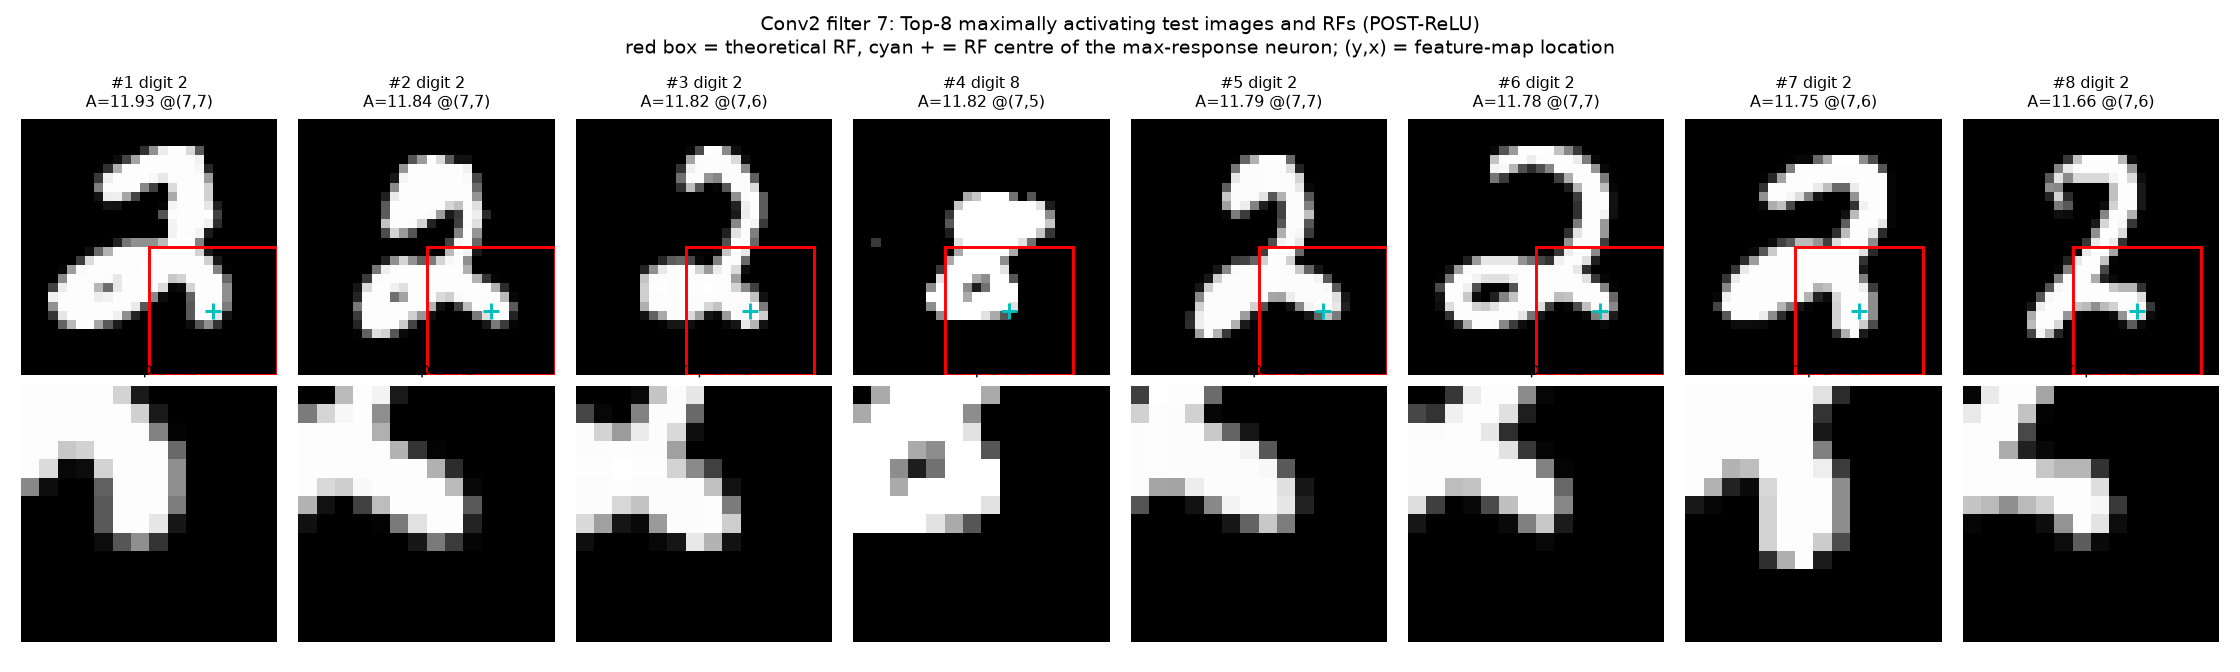
\includegraphics[width=\linewidth]{results/fig2_conv2_top8.png}
\caption{Top-8 images for Conv2 filter 7 (POST-ReLU), with the 14$\times$14 receptive field (red box) and its crop.}
\label{fig:conv2}
\end{figure}

\begin{table}[H]
\centering
\small
\begin{tabular}{cccccc}
\toprule
Rank & Test idx & Digit & Score & Location $(y,x)$ & RF region (rows, cols) \\
\midrule
1 & 218  & 2 & 11.9347 & (7,7) & 14--27, 14--27 \\
2 & 763  & 2 & 11.8351 & (7,7) & 14--27, 14--27 \\
3 & 1108 & 2 & 11.8208 & (7,6) & 14--27, 12--25 \\
4 & 1381 & 8 & 11.8187 & (7,5) & 14--27, 10--23 \\
5 & 698  & 2 & 11.7927 & (7,7) & 14--27, 14--27 \\
6 & 1789 & 2 & 11.7774 & (7,7) & 14--27, 14--27 \\
7 & 575  & 2 & 11.7518 & (7,6) & 14--27, 12--25 \\
8 & 1812 & 2 & 11.6635 & (7,6) & 14--27, 12--25 \\
\bottomrule
\end{tabular}
\caption{Top-8 for Conv2 filter 7.}
\end{table}

\textbf{Observation for Conv2 filter 7.} Seven of eight images are 2s and one is an 8. Every maximum is in the last row of the 8$\times$8 map, columns 5 to 7, so the receptive field is always the bottom-right part of the image (rows 14 to 27). In the crops there is a stroke coming down from the upper left and ending in the lower right, with background to the right. For the 2s this is the end of the base stroke, where the curve and the horizontal part meet. The 8 has a similar looking stroke. The filter therefore responds to a part of a digit made of several stroke pieces, not to a whole digit.

\textbf{Comparison.}
\begin{itemize}
\item \emph{Receptive field size.} 5$\times$5 for Conv1 and 14$\times$14 for Conv2, which is about 7.8 times the area (196 against 25 pixels).
\item \emph{Activated regions.} The Conv1 maxima are spread over the image (rows 1 to 19, columns 5 to 19 in the Experiment 2 table). The Conv2 filter 7 maxima are all in the bottom-right corner of its map. Part of this is that a 14$\times$14 field on an 8$\times$8 map covers a large share of the image, so the choice of location is coarse.
\item \emph{Pattern complexity.} The Conv1 crop is one edge, a bright stroke below a dark region. The Conv2 crop contains a long stroke, a junction or bend, and the empty space beside it.
\item \emph{Digit distribution.} Conv1 filter 2 gives 7:5 with three other digits, Conv2 filter 7 gives 2:7 with one other. This is more concentrated, but the Conv2 filters in Experiment 4 (10 and 14) are not, so I do not treat it as a rule for Conv2.
\end{itemize}

\textbf{Evidence for a change in representation.} The first piece of evidence is the field size, since Conv2 can see a bend or junction that cannot fit in 5$\times$5. The second is the crops: Conv1 patches are single edges and strokes that occur in many digits, while the Conv2 patches are made of several strokes arranged in a particular way (Figures~\ref{fig:conv1} and~\ref{fig:conv2}). The third is that Conv2 filters 5 and 7 are mostly tied to one digit, which a Conv1 filter in these results never is. This is only suggestive, because it comes from two filters and from a 2,000-image subset. Conv2 filter 7 does not draw a full 2 either, so I am not claiming that Conv2 filters represent whole digits. Also, activation values can not be compared across layers or filters (Conv1 filter 5 peaks at 2.7 while Conv2 filter 14 peaks at 26.1), because the weights and biases differ.

%%%%%%%%%%%%%%%%%%%%%%%%%%%%%%%%%%%%%%%%%%%%%%%%%%%%%%%

\section{Experiment 4: selectivity across digit classes}

\begin{figure}[H]
\centering
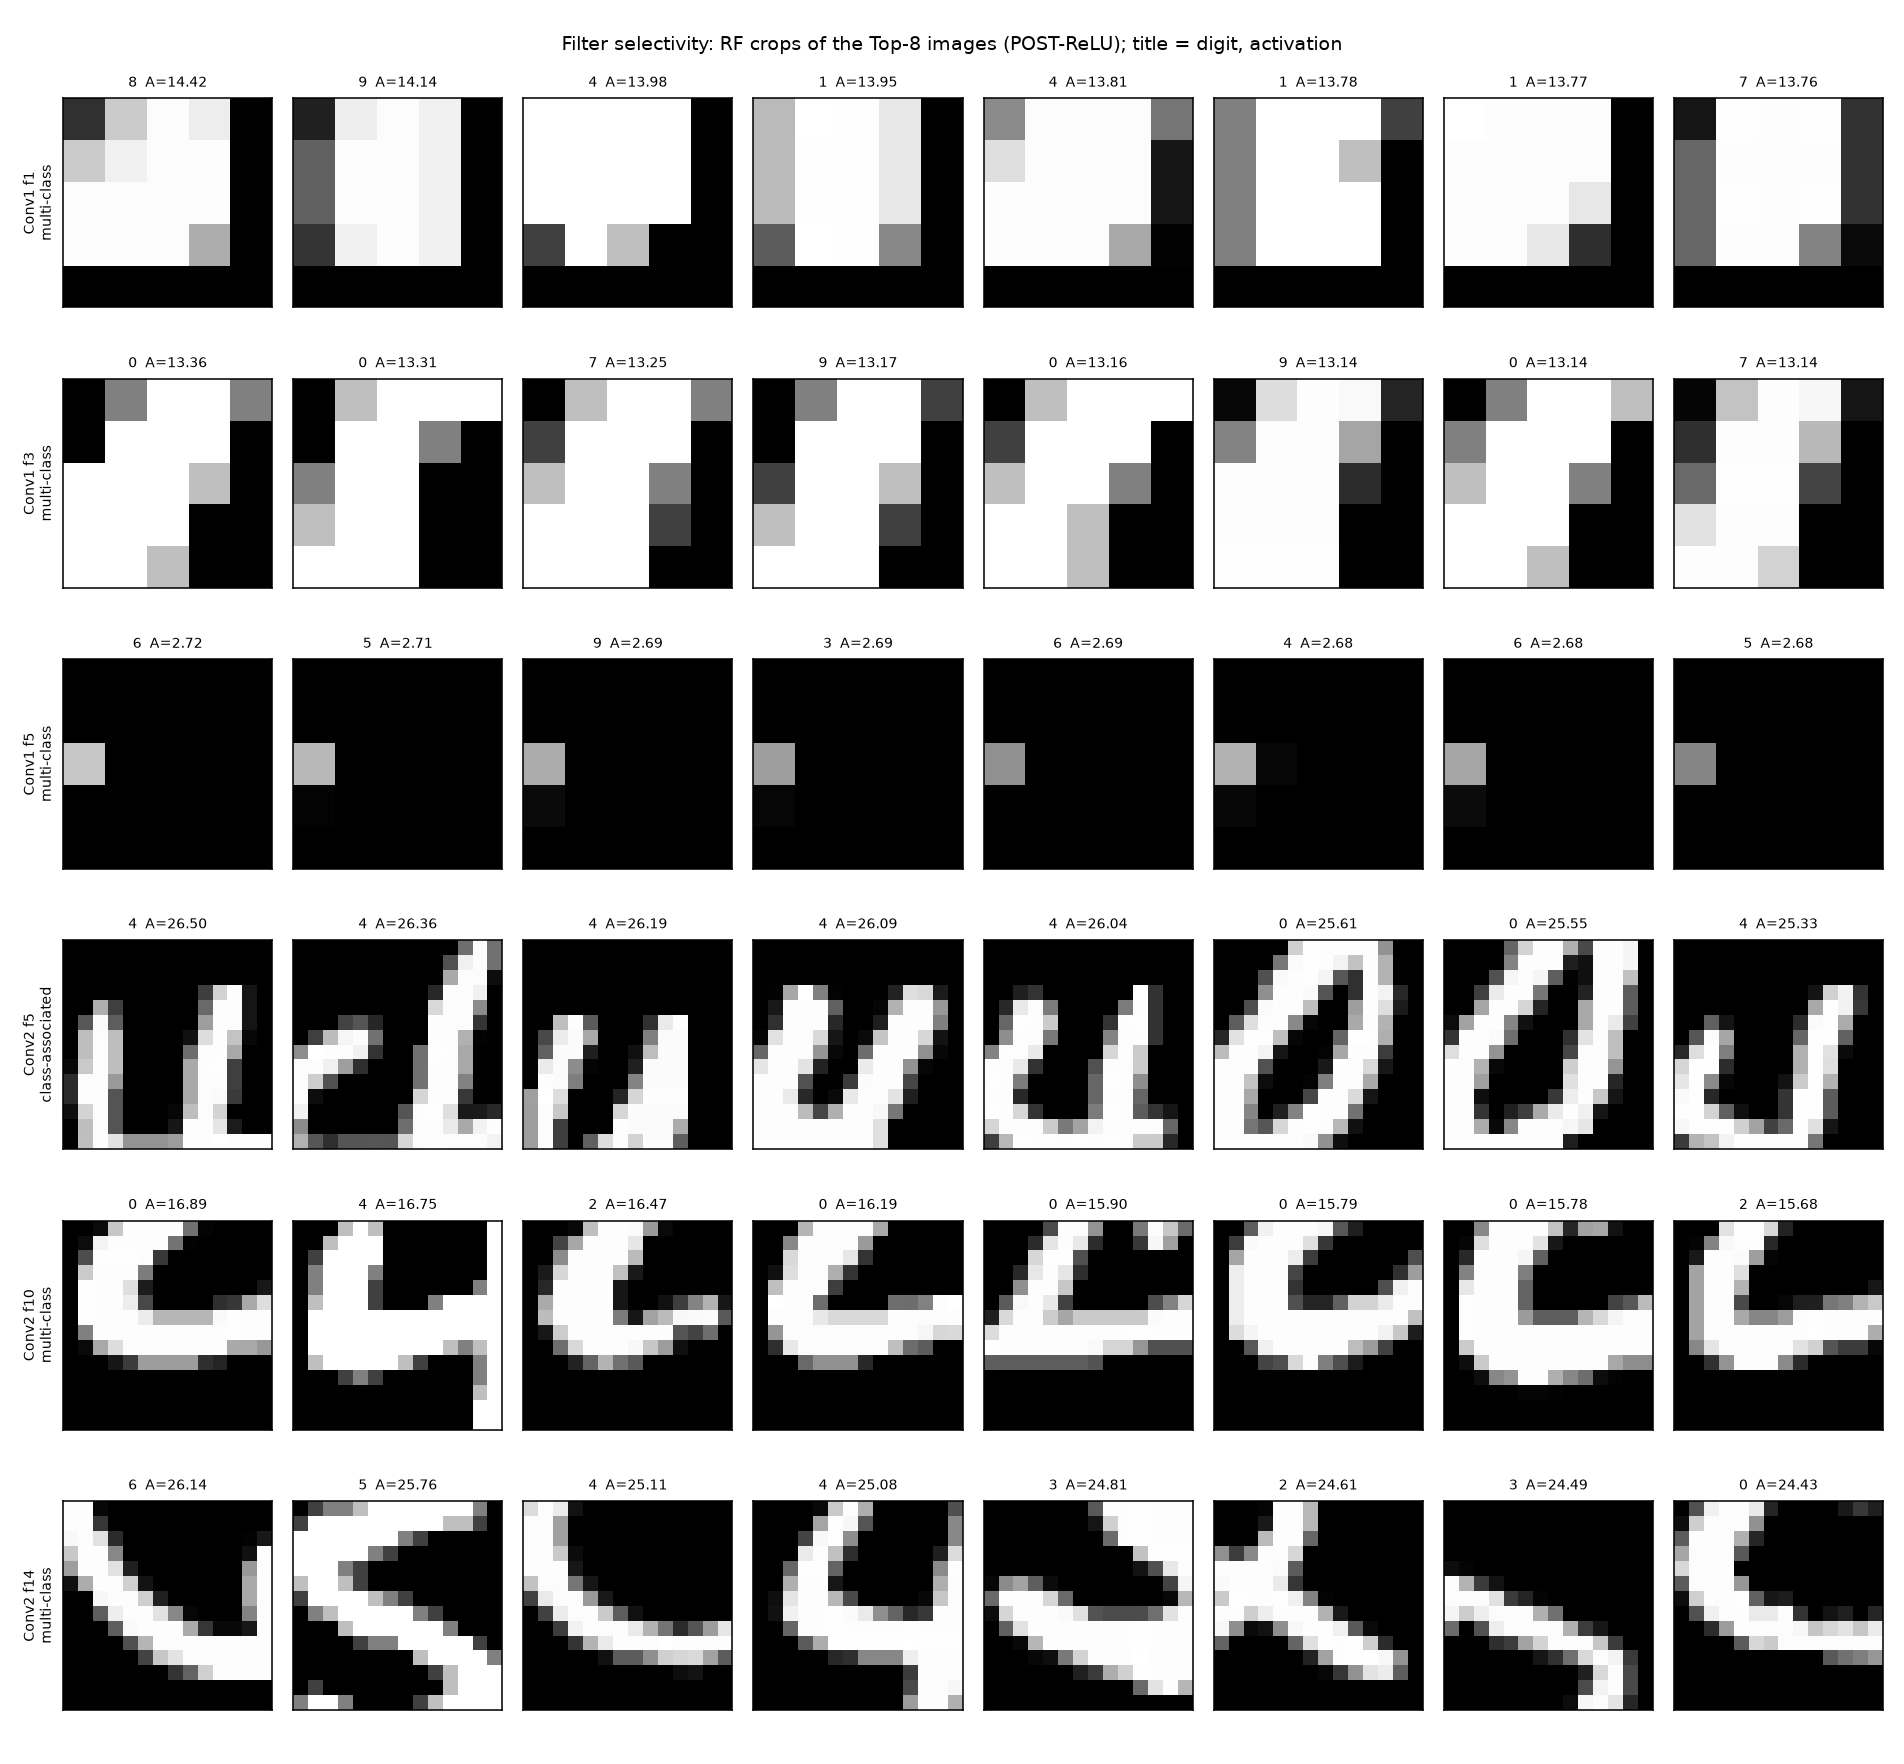
\includegraphics[width=\linewidth]{results/fig3_selectivity.png}
\caption{Receptive-field crops of the Top-8 images for three Conv1 filters (top three rows) and three Conv2 filters (bottom three rows). Each title gives the digit and the activation.}
\label{fig:sel}
\end{figure}

\begin{table}[H]
\centering
\small
\begin{tabular}{llp{3.1cm}p{4.2cm}l}
\toprule
Layer & Filter & Digits (rank order) & Activations (rank 1 to 8) & Class \\
\midrule
Conv1 & 1  & 8 9 4 1 4 1 1 7 & 14.42, 14.14, 13.98, 13.95, 13.81, 13.78, 13.77, 13.76 & multi-class \\
Conv1 & 3  & 0 0 7 9 0 9 0 7 & 13.36, 13.31, 13.25, 13.17, 13.16, 13.14, 13.14, 13.14 & multi-class \\
Conv1 & 5  & 6 5 9 3 6 4 6 5 & 2.72, 2.71, 2.69, 2.69, 2.69, 2.68, 2.68, 2.68 & multi-class \\
Conv2 & 5  & 4 4 4 4 4 0 0 4 & 26.50, 26.36, 26.19, 26.09, 26.04, 25.61, 25.55, 25.33 & class-associated \\
Conv2 & 10 & 0 4 2 0 0 0 0 2 & 16.89, 16.75, 16.47, 16.19, 15.90, 15.79, 15.78, 15.68 & multi-class \\
Conv2 & 14 & 6 5 4 4 3 2 3 0 & 26.14, 25.76, 25.11, 25.08, 24.81, 24.61, 24.49, 24.43 & multi-class \\
\bottomrule
\end{tabular}
\caption{Top-8 digit labels and activations for the six filters. The class column applies the rule from the assignment on the digit counts alone (at least 6 of 8 for class-associated; at least 3 classes and none with 6 or more for multi-class).}
\end{table}

\begin{itemize}
\item \textbf{Conv1 filter 1} (1:3, 4:2, 7, 8, 9). Multi-class by the count rule. The crops are almost entirely bright, with a dark column on the right and a dark row at the bottom, so the filter fires when a thick stroke fills most of the patch and ends on the right and bottom side. This is a shared visual pattern across digits 1, 4, 7, 8 and 9, and it is not a digit-specific feature.
\item \textbf{Conv1 filter 3} (0:4, 7:2, 9:2). Multi-class by count. The crops are mostly bright with dark pixels along the left edge and on the lower right, a stroke running roughly top to bottom through the middle of the patch. The 0s, 7s and 9s all produce this, so again the pattern is shared across digits.
\item \textbf{Conv1 filter 5} (6:3, 5:2, 3, 4, 9). Multi-class by count, but the digit labels mean little here. All 25 weights of this kernel are negative (their sum is $-5.33$) and the bias is $+0.33$, so the filter is strongest on an \emph{empty} patch: the response to a blank patch is $0.33+(-0.424)(-5.33)\approx 2.59$, and every image contains a blank patch, so every image scores at least 2.59. The Top-8 scores (2.68 to 2.72) are barely above that. All eight crops are almost black with one faint grey pixel at the left edge, which is the one position where the kernel has a positive weight ($+0.05$). So this filter detects the absence of ink, and its Top-8 is not a meaningful digit ranking.
\item \textbf{Conv2 filter 5} (4:6, 0:2). \emph{Class-associated} (6 of 8 are 4s). The crops show two roughly vertical strokes with a gap between them, which is the open-top shape of a 4. The two 0s fit the same description, since the crop catches the left and right sides of the 0. This filter looks for two parallel strokes, and the 4 is the digit that most often provides them.
\item \textbf{Conv2 filter 10} (0:5, 2:2, 4:1). Multi-class by count, with 0 the most common (5 of 8, just below the cut-off of 6). The crops share a curved stroke on the left that runs into a horizontal stroke at the bottom, with empty space in the upper right. This is common to the 0s, the 2s and the 4, so I would call it a shared pattern.
\item \textbf{Conv2 filter 14} (3:2, 4:2, and one each of 0, 2, 5, 6). The most spread out of the six: six digit classes. The crops mostly show a diagonal stroke going from upper left down to the lower right, sometimes joined to a horizontal stroke. It is a shared pattern across digits.
\end{itemize}

Overall only one of the six filters is class-associated. The Conv1 filters are multi-class and respond to the same local stroke shapes in many digits (filter 5 is an exception, it responds to empty space). Conv2 filter 5 shows that a deeper filter can lean towards one digit, but Conv2 filters 10 and 14 respond to a stroke arrangement that several digits share.

%%%%%%%%%%%%%%%%%%%%%%%%%%%%%%%%%%%%%%%%%%%%%%%%%%%%%%%

\section{Experiment 5: receptive-field analysis}

With $r_0=1$, $j_0=1$ and $r_l=r_{l-1}+(k_l-1)j_{l-1}$, $j_l=j_{l-1}s_l$:

\begin{table}[H]
\centering
\begin{tabular}{lcccc}
\toprule
Layer & $k$ & $s$ & $r_l$ & $j_l$ \\
\midrule
Input & - & - & 1 & 1 \\
Conv1 & 5 & 1 & $1+4\cdot1=5$ & 1 \\
S2 (AvgPool) & 2 & 2 & $5+1\cdot1=6$ & 2 \\
Conv2 & 5 & 1 & $6+4\cdot2=14$ & 2 \\
S4 (AvgPool) & 2 & 2 & $14+1\cdot2=16$ & 4 \\
\bottomrule
\end{tabular}
\caption{Receptive-field calculation.}
\end{table}

This gives 5$\times$5, 6$\times$6, 14$\times$14 and 16$\times$16, as the assignment asks to verify. Only Conv1 and Conv2 neurons are visualised, so 5$\times$5 and 14$\times$14 are the sizes used in the figures.

To place the field in the image: a Conv1 neuron $(y,x)$ sees input rows $y$ to $y+4$ and columns $x$ to $x+4$. For Conv2, one step in the 8$\times$8 map moves the field by $j=2$ input pixels, so neuron $(y,x)$ sees rows $2y$ to $2y+13$ and columns $2x$ to $2x+13$.

\begin{table}[H]
\centering
\begin{tabular}{lccc}
\toprule
Layer & Neuron $(y,x)$ & RF (rows, cols) & Visible part in 28$\times$28 \\
\midrule
Conv1 & (0,0)   & 0--4, 0--4     & 5$\times$5 \\
Conv1 & (12,12) & 12--16, 12--16 & 5$\times$5 \\
Conv1 & (23,23) & 23--27, 23--27 & 5$\times$5 \\
Conv2 & (0,0)   & 0--13, 0--13   & 14$\times$14 \\
Conv2 & (4,4)   & 8--21, 8--21   & 14$\times$14 \\
Conv2 & (7,7)   & 14--27, 14--27 & 14$\times$14 \\
\bottomrule
\end{tabular}
\caption{Receptive fields of corner and centre neurons.}
\end{table}

\textbf{Comparison with the figures.} The boxes in Figures~\ref{fig:conv1} and~\ref{fig:conv2} and the crops below them are 5$\times$5 and 14$\times$14, which equals the theoretical size. Even the corner neuron (7,7) of Conv2, which is used by several images in Experiment 3, has a field that ends exactly at pixel 27, so it touches the image border but does not extend past it. Because there is no padding in either convolution, no receptive field in this network goes outside the 28$\times$28 image, and the theoretical size and the visible size are the same for every neuron. The receptive field is only the region that can influence the neuron. It does not show which pixels in that region caused the response.

%%%%%%%%%%%%%%%%%%%%%%%%%%%%%%%%%%%%%%%%%%%%%%%%%%%%%%%

\section{Experiment 6: PRE-ReLU versus POST-ReLU}

Filter used: Conv2 filter 3. $S^{\mathrm{pre}}_i=\max z_i$ and $S^{\mathrm{post}}_i=\max A_i$ with $A=\max(0,z)$.

\begin{table}[H]
\centering
\small
\begin{tabular}{ccccccc}
\toprule
Rank & Test idx & Digit & $S^{\mathrm{pre}}$ & $S^{\mathrm{post}}$ & Loc.\ (PRE) & Loc.\ (POST) \\
\midrule
1 & 506  & 3 & 18.0657 & 18.0657 & (0,3) & (0,3) \\
2 & 1149 & 5 & 18.0431 & 18.0431 & (0,6) & (0,6) \\
3 & 535  & 0 & 17.9810 & 17.9810 & (6,3) & (6,3) \\
4 & 983  & 3 & 17.9751 & 17.9751 & (0,3) & (0,3) \\
5 & 1342 & 2 & 17.6932 & 17.6932 & (7,6) & (7,6) \\
6 & 1194 & 7 & 17.5969 & 17.5969 & (0,2) & (0,2) \\
7 & 302  & 3 & 17.5920 & 17.5920 & (0,2) & (0,2) \\
8 & 1499 & 5 & 17.5793 & 17.5793 & (0,3) & (0,3) \\
\bottomrule
\end{tabular}
\caption{Top-8 images by PRE-ReLU score and by POST-ReLU score. The two rankings are the same.}
\end{table}

The Top-8 sets are identical, in the same order, with the same values and the same locations. This is expected. Whenever the largest pre-activation of an image is positive, $\max_{y,x}\max(0,z)=\max_{y,x}z$, and ReLU does not change which position is the maximum. The Top-8 here all have large positive values, so ReLU makes no difference to them. Six of the eight maxima are in row 0 of the 8$\times$8 map, which means the filter responds mostly to the upper part of the image.

The two modes differ at the other end of the ranking. For 20 of the 2,000 images the PRE-ReLU maximum is negative, so every position in the map is negative. The eight lowest are listed below.

\begin{table}[H]
\centering
\small
\begin{tabular}{cccccc}
\toprule
Rank from bottom & Test idx & Digit & $S^{\mathrm{pre}}$ & $S^{\mathrm{post}}$ & Loc.\ of PRE max \\
\midrule
1 & 1195 & 1 & $-0.5686$ & 0 & (3,1) \\
2 & 1631 & 1 & $-0.5361$ & 0 & (3,6) \\
3 & 1061 & 1 & $-0.4972$ & 0 & (7,5) \\
4 & 479  & 1 & $-0.4930$ & 0 & (7,3) \\
5 & 1993 & 1 & $-0.3780$ & 0 & (7,1) \\
6 & 915  & 1 & $-0.3759$ & 0 & (7,1) \\
7 & 1532 & 1 & $-0.2970$ & 0 & (3,6) \\
8 & 1240 & 1 & $-0.2714$ & 0 & (7,1) \\
\bottomrule
\end{tabular}
\caption{The eight lowest-scoring images. The PRE value is the least negative response in the map, not a positive activation.}
\end{table}

All eight are the digit 1. The listed locations are just where the least negative value happened to be. They should not be read as where the filter ``fires'', because it does not fire anywhere on these images. In the POST-ReLU map these images all have $S^{\mathrm{post}}=0$, so they tie with each other and the ordering between them is lost (it is arbitrary in my code, which keeps the original image order). The PRE-ReLU score still keeps an order for them.

\textbf{Why POST-ReLU is convenient.} ReLU sets every negative value to zero and keeps positive values unchanged, so the map contains only evidence that the filter's pattern is present, and ``0'' means ``not present''. With PRE-ReLU values, a large negative number could be misread as strong activity, even though it means the pattern is absent or opposite. POST-ReLU is also the value that gets passed to the next layer, so it is the response that matters for the rest of the network. The cost is that the information about how negative the response was is discarded.

%%%%%%%%%%%%%%%%%%%%%%%%%%%%%%%%%%%%%%%%%%%%%%%%%%%%%%%

\section{Conclusion}

The network reached 98.55\% test accuracy on the 2,000-image test set. The theoretical receptive fields come out as 5$\times$5 for Conv1 and 14$\times$14 for Conv2, and they match the regions in the figures. Conv1 filters respond to short edges and strokes that appear in many digits. The Conv2 filters I looked at respond to combinations of strokes, and one of them (filter 5) mostly picks out 4s. None of them is a full digit detector. PRE-ReLU and POST-ReLU give the same Top-8 for the filter tested, and they only differ for images where every response is negative. All of the selected filters, and the 2,000-image scan, were my own choices, so the specific digits and values will change if the assigned filters or the full test set are used.

\end{document}
